\documentclass[12pt,a4paper]{report}
\input{00 - preambule}

\begin{document}

\chapter{Fonctions trigonométriques}

\section{Arcsin}
\begin{definition}{Arcsinus}{}
Soit $S : t\in \left[-\dfrac{\pi}{2}, \dfrac{\pi}{2}\right] \mapsto \sin t \in [-1,1]$\\
$S$ est continue strictement croissante sur $\left[-\dfrac{\pi}{2}, \dfrac{\pi}{2}\right]$ et $S\left(\left[-\dfrac{\pi}{2}, \dfrac{\pi}{2}\right]\right) = \left[ S\left(-\dfrac{\pi}{2}\right),S\left(\dfrac{\pi}{2}\right)\right] = [-1,1]$\\
$S$ est donc \strong{bijective}. Par définition, \textbox{$\arcsin$ = $S^{-1}$}
\end{definition}

\begin{remarque}[Dérivabilité]
On sait que $\arcsin$ est aussi continue strictement croissante. \\
De plus, $S$ est dérivable sur $\left[-\dfrac{\pi}{2}, \dfrac{\pi}{2}\right]$ et $S'(t)= \cos t$\\
D'où : 
\begin{center}
    $\forall t \in \left[-\dfrac{\pi}{2}, \dfrac{\pi}{2}\right]$, $S'(t) > 0$
\end{center}
Donc $\arcsin$ est dérivable sur $S\left(\left]-\dfrac{\pi}{2}, \dfrac{\pi}{2}\right[\right) = ]-1,1[$
\end{remarque}

\begin{propositions}{Arcsin - Dérivée}{}
Pour $x\in ]-1,1[$ : 
\begin{center}
    $\arcsin'(x) = \dfrac{1}{\sin'(\arcsin x)} = $ $\dfrac{1}{\cos(\arcsin x)}$
\end{center}
On a, pour $-1 \leq x \leq 1$ : 
\begin{center}
    $\cos^2(\arcsin(x)+\underbrace{\sin^2(\arcsin x)}_{x^2}=1$\\
    $\cos (\arcsin x) = \pm \sqrt{1-x^2}$
\end{center}
Or, $\arcsin x \in \left[-\dfrac{\pi}{2}, \dfrac{\pi}{2}\right]$, donc $\cos (\arcsin x)\geq 0$
\begin{center}
    \textbox{$\cos (\arcsin x) = + \sqrt{1-x^2}$}
\end{center}
Donc pour $-1<x<1$ : \textbox{$\arcsin'(x)=\dfrac{1}{\sqrt{1-x^2}}$}
\end{propositions}

\begin{remarque}[Remarques]
\begin{itemize}
    \item On voit donc que $\arcsin'$ est $C^\infty$ sur $]-1,1[$, donc $\arcsin$ aussi 
    \item $\arcsin'x \xrightarrow[x \to 1^-]{} + \infty$\\
    $\left(\text{Donc d'après le théorème \textit{"limite de la dérivée"},} \dfrac{\arcsin x - \arcsin 1}{x-1} \xrightarrow[x\to 1^-]{} + \infty\right)$\\
    $\arcsin 1 = \dfrac{\pi}{2}$ ( car $S(\frac{\pi}{2})=1$ ) $\Longrightarrow$ tangente verticale au graphe de $\arcsin$ au point $\left(1,\dfrac{\pi}{2}\right)$\\
    De même, $\arcsin'x \xrightarrow[x \to 1^+]{} - \infty$
    \item Pour $x,y \in \R$, $y= \arcsin x \Longleftrightarrow y\in \left[-\dfrac{\pi}{2}, \dfrac{\pi}{2}\right], x \in [-1,1], \mathbox{x = \sin y}$
    \item Pour $t\in [-1,1]$, $\sin(\arcsin t)= S\circ S^{-1} (t)=t$
    \item Pour $\theta \in \R$, $\arcsin (\sin \theta)= \theta$ \textbf{uniquement si} $\theta \in \left[-\dfrac{\pi}{2}, \dfrac{\pi}{2}\right]$\\
    Par exemple : 
    \begin{center}
        $\arcsin \left(\sin \dfrac{2\pi}{3} \right)=\arcsin \left(\dfrac{\sqrt{3}}{2}\right)=\dfrac{\pi}{3}$
    \end{center}
\end{itemize}
\end{remarque}

\begin{propositions}{Arcsin - Impaire}{}
Soit $x\in [-1,1]$, $\theta=\arcsin x$ alors $\theta \in \left[-\dfrac{\pi}{2}, \dfrac{\pi}{2}\right]$ donc $-\theta \in \left[-\dfrac{\pi}{2}, \dfrac{\pi}{2}\right]$ et $\sin (-\theta) = -\sin \theta = -x$
\begin{center}
    \textbox{$-\theta = \arcsin(-x)$}
\end{center}
\end{propositions}

\begin{remarque}[Valeurs remarquables]
\begin{center}
    \begin{tabular}{|Sc|Sc|Sc|Sc|Sc|Sc|}
      \hline
      $x$ & $0$ & $\dfrac{1}{2}$ & $\dfrac{\sqrt{2}}{2}$ & $\dfrac{\sqrt{3}}{2}$ & $1$\\
      \hline
      $\arcsin x$ & $0$ & $\dfrac{\pi}{6}$ & $\dfrac{\pi}{4}$ & $\dfrac{\pi}{3}$ & $\dfrac{\pi}{2}$\\
      \hline
     \end{tabular}
     \\
\end{center}
\end{remarque}

\begin{remarque}[Graphique associé]
\begin{center}
    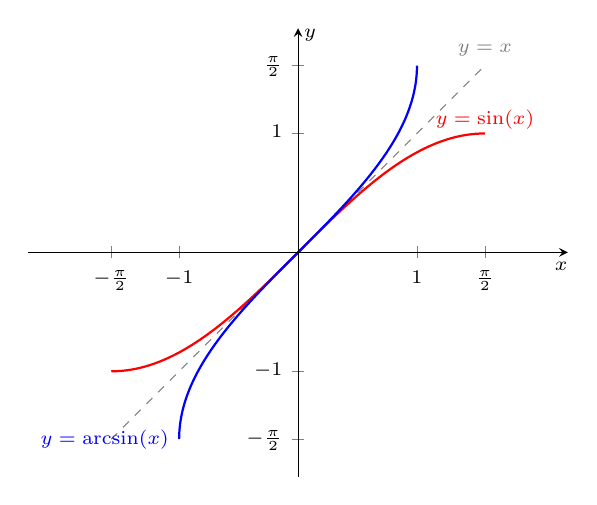
\begin{tikzpicture}[>=stealth]
  \begin{axis}
    [
      axis on top, 
      font=\scriptsize,
      typeset ticklabels with strut, 
      unit vector ratio = 1 1,
      samples = 201,
      axis lines = center,
      xlabel = {$x$},
      ylabel = {$y$},
      xtick={-pi/2,-1,0,1,pi/2},
      xticklabels={$-\frac{\pi}{2}$,$-1$,$0$,$1$,$\frac{\pi}{2}$},
      ticklabel style = {fill=white, fill opacity=.7,text opacity=1},
      ytick={-pi/2,-1,0,1,pi/2},
      yticklabels={$-\frac{\pi}{2}$,$-1$,$0$,$1$,$\frac{\pi}{2}$},
      domain=-pi/2:pi/2,
      x label style={at={(current axis.right of origin)}, anchor=north east,inner xsep=0pt},
      y label style={at={(current axis.above origin)}, anchor=north west,inner ysep=0pt, inner xsep=1pt, xshift=1pt},
      enlarge y limits=.1,
    ]
    \draw[gray, dashed] (-pi/2,-pi/2) -- (pi/2,pi/2) node[above, at end] {$y = x$};
    \addplot[red, thick] {sin(deg(x))} 
      node [at end, anchor = south,inner ysep=1pt] {$y=\sin(x)$} ;
    \addplot[blue, thick] (sin(deg(x)),x) 
      node [at start, anchor = east] {$y=\arcsin(x)$} ;
  \end{axis}
\end{tikzpicture}
\end{center}
\end{remarque}


\section{Arccos}

\begin{definition}{Arcsinus}{}
Soit $C : t\in \left[0, \pi \right] \mapsto \cos t \in [-1,1]$\\
$C$ est continue strictement décroissante et $C\left(\left[0, \pi\right]\right) = [ C(\pi),C(0)] = [-1,1]$\\
$C$ est donc \strong{bijective}. Par définition, \textbox{$\arccos$ = $C^{-1} : [-1,1] \to [0,\pi]$}
\end{definition}

\begin{remarque}[Dérivabilité]
On sait que $\arccos$ est continue strictement décroissante. \\
De plus, $C$ est dérivable sur $\left[0, \pi \right]$ et $C'(t)= - \sin t$\\
D'où : 
\begin{center}
    Pour $0<t<\pi$, $C'(t) \neq 0$
\end{center}
Donc $\arccos$ est dérivable sur $C\left(\left]0, \pi \right[\right) = ]-1,1[$
\end{remarque}

\begin{propositions}{Arccos - Dérivée}{}
Pour $x\in ]-1,1[$ : 
\begin{center}
    $\arccos'(x) = \dfrac{1}{\cos'(\arccos x)} = $ $ - \dfrac{1}{\sin(\arccos x)}$
\end{center}
On a, pour $-1 \leq x \leq 1$ : 
\begin{center}
    $\underbrace{\cos^2(\arccos x)}_{x^2}+\sin^2(\arccos x)=1$\\
    $\sin (\arccos x) = \pm \sqrt{1-x^2}$
\end{center}
Or, $\arccos x \in \left[0, \pi\right]$, donc $\sin (\arccos x)\geq 0$
\begin{center}
    \textbox{$\sin (\arccos x) = + \sqrt{1-x^2}$}
\end{center}
Donc pour $-1<x<1$ : \textbox{$\arccos'(x)=-\dfrac{1}{\sqrt{1-x^2}}$}
\end{propositions}

\begin{remarque}
\begin{itemize}
    \item Pour $x,y \in \R$, $y= \arccos x \Longleftrightarrow y\in [0,\pi], x \in [-1,1]$, \strong{$x = \cos y$}
    \item Soit $\varphi : x \in [-1,1] \to \arcsin x + \arccos x \in \R$\\
    $\varphi$ est continue sur $[-1,1]$, dérivable sur $]-1,1[$ et $\forall x \in ]-1,1[$, $\varphi(0)=\dfrac{\pi}{2}$\\
    Donc $\mathbox{\forall x \in [-1,1], \arccos x = \dfrac{\pi}{2} - \arcsin x}$\\
    \\
    \item Soit $x \in [-1,1]$, $\theta=\arcsin x \in \left[-\dfrac{\pi}{2}, \dfrac{\pi}{2}\right]$ alors $\dfrac{\pi}{2}-\theta \in [0,\pi]$ et $\cos \left (\dfrac{\pi}{2} - \theta\right)=\sin \theta = x$\\
    Donc \strong{$\dfrac{\pi}{2} - \theta = \arccos x$}
\end{itemize}
\end{remarque}

\begin{remarque}[Valeurs remarquables]
\begin{center}
    \begin{tabular}{|Sc|Sc|Sc|Sc|Sc|Sc|Sc|Sc|Sc|Sc|}
      \hline
      $x$ & $-1$ & $-\dfrac{\sqrt{3}}{2}$ & $-\dfrac{\sqrt{2}}{2}$ & $-\dfrac{1}{2}$ & $0$ & $\dfrac{1}{2}$ & $\dfrac{\sqrt{2}}{2}$ & $\dfrac{\sqrt{3}}{2}$ & $1$\\
      \hline
      $\arccos x$ & $\pi$ & $\dfrac{5\pi}{6}$ & $\dfrac{3\pi}{4}$ & $\dfrac{2\pi}{3}$ & $\dfrac{\pi}{2}$ & $\dfrac{\pi}{3}$ & $\dfrac{\pi}{4}$ & $\dfrac{\pi}{6}$ & $0$\\
      \hline
     \end{tabular}
     \\
\end{center}
\end{remarque}

\begin{remarque}[Graphique associé]
\begin{center}
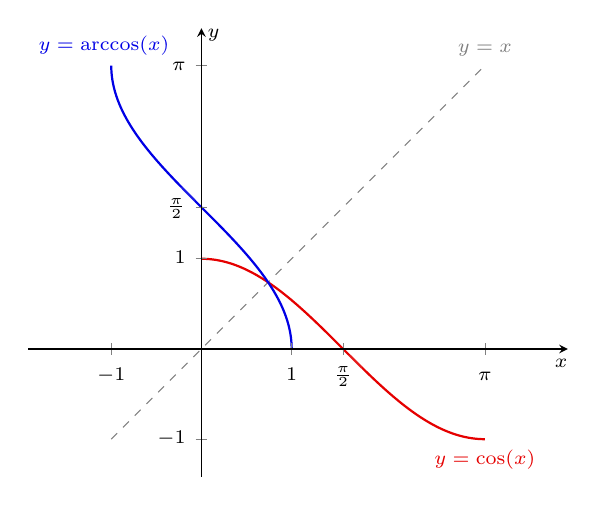
\begin{tikzpicture}[>=stealth]
  \begin{axis}
    [
      axis on top, 
      font=\scriptsize,
      typeset ticklabels with strut,
      unit vector ratio = 1 1,
      samples = 201,
      axis lines = center,
      xlabel = {$x$},
      ylabel = {$y$},
      xtick={-1, 0, 1, pi/2, pi},
      xticklabels={$-1$, $0$,$1$,$\frac{\pi}{2}$, $\pi$},
      ticklabel style = {fill=white, fill opacity=.1, text opacity=1},
      ytick={-pi/2, -1, 0, 1, pi/2, pi},
      yticklabels={$-\frac{\pi}{2}$,$-1$,$0$,$1$,$\frac{\pi}{2}$, $\pi$},
      domain=0:pi,
      x label style={at={(current axis.right of origin)}, anchor=north east,inner xsep=0pt},
      y label style={at={(current axis.above origin)}, anchor=north west,inner ysep=0pt, inner xsep=1pt, xshift=1pt},
      enlarge y limits=.1,
    ]

    \draw[gray, dashed] (-1,-1) -- (pi,pi) node[above, at end] {$y = x$};
    \addplot[red!90!black, thick] {cos(deg(x))}
    node [at end, anchor = north] {$y=\cos(x)$} ;
    \addplot[blue!90!black, thick] (cos(deg(x)),x) 
    node [at end, anchor=-70] {$y=\arccos(x)$} ;
  \end{axis}
\end{tikzpicture}
\end{center}
\end{remarque}

\section{Arctan}
\begin{definition}{Arctan}{}
Soit $T : t\in \left]-\dfrac{\pi}{2}, \dfrac{\pi}{2}\right[ \mapsto \tan t \in \R$\\
$T$ est continue strictement croissante et $T\left(\left]-\dfrac{\pi}{2}, \dfrac{\pi}{2}\right[\right) = \left]\displaystyle \lim_{\frac{-\pi}{2}^+} \tan,\displaystyle \lim_{\frac{\pi}{2}^-} \tan \right[ = ]-\infty,\infty[ = \R$\\
$T$ est donc \strong{bijective}. Par définition, \textbox{$\arctan$ = $T^{-1}$}
\end{definition}

\begin{remarque}[Dérivabilité]
On sait que $\arctan$ est bijective, continue strictement croissante de $\R$ dans $\left]-\dfrac{\pi}{2}, \dfrac{\pi}{2}\right[$. \\
Pour $\theta$, $t \in \R$
\begin{center}
    $\theta=\arctan t$ $\Longleftrightarrow$ $\theta \in \left]-\dfrac{\pi}{2}, \dfrac{\pi}{2}\right[$ et $t = \tan \theta$
\end{center}
De plus, $T$ est dérivable ( et même $C^\infty$) : $\forall t \in \left]-\dfrac{\pi}{2}, \dfrac{\pi}{2}\right[, T'(x)=1+\tan^2 t >0$\\
Donc $\arctan$ est de classe $C^\infty \in \R$
\end{remarque}

\begin{propositions}{Arctan - Dérivée}{}
\begin{center}
    $\forall x \in \R$, $\arctan'(x)=\dfrac{1}{T'(\arctan x)} = \dfrac{1}{1+\tan^2\arctan x} = \dfrac{1}{1+x^2}$
\end{center}
\end{propositions}

\begin{remarque}[Valeurs remarquables]
\begin{center}
    \begin{tabular}{|Sc|Sc|Sc|Sc|Sc|}
      \hline
      $x$ & $0$ & $\dfrac{1}{\sqrt{3}}$ & $1$ & $\sqrt{3}$\\
      \hline
      $\arctan x$ & $0$ & $\dfrac{\pi}{6}$ & $\dfrac{\pi}{4}$ & $\dfrac{\pi}{3}$\\
      \hline
     \end{tabular}
     \\
\end{center}
\end{remarque}

\begin{remarque}[Graphique associé]
\begin{center}
    \textit{Graphique à venir ...}
\end{center}
\end{remarque}
\end{document}
